% Options for packages loaded elsewhere
\PassOptionsToPackage{unicode}{hyperref}
\PassOptionsToPackage{hyphens}{url}
%
\documentclass[
]{book}
\usepackage{amsmath,amssymb}
\usepackage{lmodern}
\usepackage{iftex}
\ifPDFTeX
  \usepackage[T1]{fontenc}
  \usepackage[utf8]{inputenc}
  \usepackage{textcomp} % provide euro and other symbols
\else % if luatex or xetex
  \usepackage{unicode-math}
  \defaultfontfeatures{Scale=MatchLowercase}
  \defaultfontfeatures[\rmfamily]{Ligatures=TeX,Scale=1}
\fi
% Use upquote if available, for straight quotes in verbatim environments
\IfFileExists{upquote.sty}{\usepackage{upquote}}{}
\IfFileExists{microtype.sty}{% use microtype if available
  \usepackage[]{microtype}
  \UseMicrotypeSet[protrusion]{basicmath} % disable protrusion for tt fonts
}{}
\makeatletter
\@ifundefined{KOMAClassName}{% if non-KOMA class
  \IfFileExists{parskip.sty}{%
    \usepackage{parskip}
  }{% else
    \setlength{\parindent}{0pt}
    \setlength{\parskip}{6pt plus 2pt minus 1pt}}
}{% if KOMA class
  \KOMAoptions{parskip=half}}
\makeatother
\usepackage{xcolor}
\usepackage{color}
\usepackage{fancyvrb}
\newcommand{\VerbBar}{|}
\newcommand{\VERB}{\Verb[commandchars=\\\{\}]}
\DefineVerbatimEnvironment{Highlighting}{Verbatim}{commandchars=\\\{\}}
% Add ',fontsize=\small' for more characters per line
\usepackage{framed}
\definecolor{shadecolor}{RGB}{248,248,248}
\newenvironment{Shaded}{\begin{snugshade}}{\end{snugshade}}
\newcommand{\AlertTok}[1]{\textcolor[rgb]{0.94,0.16,0.16}{#1}}
\newcommand{\AnnotationTok}[1]{\textcolor[rgb]{0.56,0.35,0.01}{\textbf{\textit{#1}}}}
\newcommand{\AttributeTok}[1]{\textcolor[rgb]{0.77,0.63,0.00}{#1}}
\newcommand{\BaseNTok}[1]{\textcolor[rgb]{0.00,0.00,0.81}{#1}}
\newcommand{\BuiltInTok}[1]{#1}
\newcommand{\CharTok}[1]{\textcolor[rgb]{0.31,0.60,0.02}{#1}}
\newcommand{\CommentTok}[1]{\textcolor[rgb]{0.56,0.35,0.01}{\textit{#1}}}
\newcommand{\CommentVarTok}[1]{\textcolor[rgb]{0.56,0.35,0.01}{\textbf{\textit{#1}}}}
\newcommand{\ConstantTok}[1]{\textcolor[rgb]{0.00,0.00,0.00}{#1}}
\newcommand{\ControlFlowTok}[1]{\textcolor[rgb]{0.13,0.29,0.53}{\textbf{#1}}}
\newcommand{\DataTypeTok}[1]{\textcolor[rgb]{0.13,0.29,0.53}{#1}}
\newcommand{\DecValTok}[1]{\textcolor[rgb]{0.00,0.00,0.81}{#1}}
\newcommand{\DocumentationTok}[1]{\textcolor[rgb]{0.56,0.35,0.01}{\textbf{\textit{#1}}}}
\newcommand{\ErrorTok}[1]{\textcolor[rgb]{0.64,0.00,0.00}{\textbf{#1}}}
\newcommand{\ExtensionTok}[1]{#1}
\newcommand{\FloatTok}[1]{\textcolor[rgb]{0.00,0.00,0.81}{#1}}
\newcommand{\FunctionTok}[1]{\textcolor[rgb]{0.00,0.00,0.00}{#1}}
\newcommand{\ImportTok}[1]{#1}
\newcommand{\InformationTok}[1]{\textcolor[rgb]{0.56,0.35,0.01}{\textbf{\textit{#1}}}}
\newcommand{\KeywordTok}[1]{\textcolor[rgb]{0.13,0.29,0.53}{\textbf{#1}}}
\newcommand{\NormalTok}[1]{#1}
\newcommand{\OperatorTok}[1]{\textcolor[rgb]{0.81,0.36,0.00}{\textbf{#1}}}
\newcommand{\OtherTok}[1]{\textcolor[rgb]{0.56,0.35,0.01}{#1}}
\newcommand{\PreprocessorTok}[1]{\textcolor[rgb]{0.56,0.35,0.01}{\textit{#1}}}
\newcommand{\RegionMarkerTok}[1]{#1}
\newcommand{\SpecialCharTok}[1]{\textcolor[rgb]{0.00,0.00,0.00}{#1}}
\newcommand{\SpecialStringTok}[1]{\textcolor[rgb]{0.31,0.60,0.02}{#1}}
\newcommand{\StringTok}[1]{\textcolor[rgb]{0.31,0.60,0.02}{#1}}
\newcommand{\VariableTok}[1]{\textcolor[rgb]{0.00,0.00,0.00}{#1}}
\newcommand{\VerbatimStringTok}[1]{\textcolor[rgb]{0.31,0.60,0.02}{#1}}
\newcommand{\WarningTok}[1]{\textcolor[rgb]{0.56,0.35,0.01}{\textbf{\textit{#1}}}}
\usepackage{longtable,booktabs,array}
\usepackage{calc} % for calculating minipage widths
% Correct order of tables after \paragraph or \subparagraph
\usepackage{etoolbox}
\makeatletter
\patchcmd\longtable{\par}{\if@noskipsec\mbox{}\fi\par}{}{}
\makeatother
% Allow footnotes in longtable head/foot
\IfFileExists{footnotehyper.sty}{\usepackage{footnotehyper}}{\usepackage{footnote}}
\makesavenoteenv{longtable}
\usepackage{graphicx}
\makeatletter
\def\maxwidth{\ifdim\Gin@nat@width>\linewidth\linewidth\else\Gin@nat@width\fi}
\def\maxheight{\ifdim\Gin@nat@height>\textheight\textheight\else\Gin@nat@height\fi}
\makeatother
% Scale images if necessary, so that they will not overflow the page
% margins by default, and it is still possible to overwrite the defaults
% using explicit options in \includegraphics[width, height, ...]{}
\setkeys{Gin}{width=\maxwidth,height=\maxheight,keepaspectratio}
% Set default figure placement to htbp
\makeatletter
\def\fps@figure{htbp}
\makeatother
\setlength{\emergencystretch}{3em} % prevent overfull lines
\providecommand{\tightlist}{%
  \setlength{\itemsep}{0pt}\setlength{\parskip}{0pt}}
\setcounter{secnumdepth}{5}
\usepackage{booktabs}
\ifLuaTeX
  \usepackage{selnolig}  % disable illegal ligatures
\fi
\usepackage[]{natbib}
\bibliographystyle{apalike}
\IfFileExists{bookmark.sty}{\usepackage{bookmark}}{\usepackage{hyperref}}
\IfFileExists{xurl.sty}{\usepackage{xurl}}{} % add URL line breaks if available
\urlstyle{same} % disable monospaced font for URLs
\hypersetup{
  pdftitle={JAMES Documentation},
  pdfauthor={Stef van Buuren, Arjan Huizing},
  hidelinks,
  pdfcreator={LaTeX via pandoc}}

\title{JAMES Documentation}
\author{Stef van Buuren, Arjan Huizing}
\date{2023-05-26}

\begin{document}
\maketitle

{
\setcounter{tocdepth}{1}
\tableofcontents
}
\hypertarget{preface}{%
\chapter*{Preface}\label{preface}}
\addcontentsline{toc}{chapter}{Preface}

Hi, welcome to JAMES!

This document contains documentation of the Joint Automatic Measurement and Evaluation System (JAMES). JAMES is fully programmed in \texttt{R} and makes it functionality available as an API running under \texttt{OpenCPU}.

This contents of the file is fully in the works. It is it neither complete nor garanteed to be accurate, consider it as a journey guide for your travel through JAMES. Nevertheless, I hope that it will help to understand basic ideas, technologies and applications.

Last version: June 2021.

\hypertarget{intro}{%
\chapter{Introduction}\label{intro}}

\hypertarget{overview}{%
\section{Overview}\label{overview}}

This chapter gives a brief overview the Joint Automatic Measurement and Evaluation System (JAMES).

JAMES is an experimental web service for creating and interpreting charts of child growth and
development. The current version

\begin{enumerate}
\def\labelenumi{\arabic{enumi}.}
\tightlist
\item
  provides access to high-quality over 300 growth charts used by the Dutch youth health care;
\item
  interchanges data coded according to the \href{https://www.ncj.nl/themadossiers/informatisering/basisdataset/documentatie/?cat=13}{Basisdataset JGZ};
\item
  screens for abnormal height, weight and head circumference;
\item
  converts developmental data into the D-score;
\item
  plot D-scores on special D-score charts;
\item
  predicts future growth and development.
\end{enumerate}

The service can be used by anyone interested in high-quality charts for monitoring and evaluating childhood growth and development. This chapter highlights the components of JAMES.

\hypertarget{architecture}{%
\section{Architecture}\label{architecture}}

JAMES provides its services through \href{https://www.opencpu.org}{OpenCPU}, an open system for scientific computing and reproducible research. The system allows for easy integration of growth charts into any \texttt{HTTPS} compliant client by means of OpenCPU's \href{https://www.opencpu.org/api.html}{API}. The JAMES webservice is a RESTful Application Programming Interface (API).

The contents of the system consist of two parts:

\begin{itemize}
\tightlist
\item
  \textbf{JAMES}: A collection of R packages that provides back-end functionality
\item
  \textbf{JESSE}: A gateway front-end JAMES that translates incoming and outcoming requests (not yet realised)
\end{itemize}

\hypertarget{r-packages}{%
\section{R packages}\label{r-packages}}

\hypertarget{james-active-packages}{%
\subsection{JAMES Active packages}\label{james-active-packages}}

Active packages reside on the JAMES server and provide all functionality.

\begin{longtable}[]{@{}
  >{\raggedright\arraybackslash}p{(\columnwidth - 4\tabcolsep) * \real{0.1268}}
  >{\raggedright\arraybackslash}p{(\columnwidth - 4\tabcolsep) * \real{0.0845}}
  >{\raggedright\arraybackslash}p{(\columnwidth - 4\tabcolsep) * \real{0.7887}}@{}}
\toprule()
\begin{minipage}[b]{\linewidth}\raggedright
Package
\end{minipage} & \begin{minipage}[b]{\linewidth}\raggedright
Open
\end{minipage} & \begin{minipage}[b]{\linewidth}\raggedright
Description
\end{minipage} \\
\midrule()
\endhead
\href{https://github.com/growthcharts/james}{\texttt{james}} & Y & Joint Automatic Measurement and Evaluation System \\
\href{https://github.com/growthcharts/nlreferences}{\texttt{nlreferences}} & Y & Growth References for Children living in The Netherlands \\
\href{https://github.com/growthcharts/centile}{\texttt{centile}} & Y & Translate Measurements, Z-Scores and Centiles with the RIF format \\
\href{https://github.com/growthcharts/chartbox}{\texttt{chartbox}} & Y & Collection of Growth Charts \\
\href{https://github.com/growthcharts/chartcatalog}{\texttt{chartcatalog}} & Y & Catalog of JAMES Growth Charts \\
\href{https://github.com/growthcharts/chartplotter}{\texttt{chartplotter}} & N & Analysing and Plotting Growth Curves \\
\href{https://github.com/growthcharts/curvematching}{\texttt{curvematching}} & N & Personalised Prediction by Matching Invididuals \\
\href{https://github.com/growthcharts/donorloader}{\texttt{donorloader}} & N & Loads Donor Data from Package or Database \\
\href{https://github.com/growthcharts/brokenstick}{\texttt{brokenstick}} & Y & Broken Stick Model for Irregular Longitudinal Data \\
\href{https://github.com/D-score/dscore}{\texttt{dscore}} & Y & D-Score for Child Development \\
\href{https://github.com/growthcharts/bdsreader}{\texttt{bdsreader}} & Y & Read Data from the Basisdataset Jeugdgezondheidszorg \\
\href{https://github.com/growthcharts/growthscreener}{\texttt{growthscreener}} & Y & Finding Children with Unusual Growth Patterns \\
\href{https://github.com/growthcharts/jamesclient}{\texttt{jamesclient}} & Y & Client-side R Functions for JAMES \\
\href{https://github.com/growthcharts/jamesdemodata}{\texttt{jamesdemodata}} & Y & Demo Data for JAMES \\
\bottomrule()
\end{longtable}

\hypertarget{james-support-packages}{%
\subsection{JAMES Support packages}\label{james-support-packages}}

Support packages produce half-fabricated materials, provide testing or store documentation.

\begin{longtable}[]{@{}
  >{\raggedright\arraybackslash}p{(\columnwidth - 4\tabcolsep) * \real{0.1268}}
  >{\raggedright\arraybackslash}p{(\columnwidth - 4\tabcolsep) * \real{0.0845}}
  >{\raggedright\arraybackslash}p{(\columnwidth - 4\tabcolsep) * \real{0.7887}}@{}}
\toprule()
\begin{minipage}[b]{\linewidth}\raggedright
Package
\end{minipage} & \begin{minipage}[b]{\linewidth}\raggedright
Open
\end{minipage} & \begin{minipage}[b]{\linewidth}\raggedright
Description
\end{minipage} \\
\midrule()
\endhead
\href{https://github.com/stefvanbuuren/donordata}{\texttt{donordata}} & N & Longitudinal Data for Curve Matching \\
\href{https://github.com/stefvanbuuren/chartdesigner}{\texttt{chartdesigner}} & N & Design Growth Charts for JAMES \\
\href{https://github.com/stefvanbuuren/gateway}{\texttt{gateway}} & N & Entry to TNO online analytic growth modules \\
\href{https://github.com/growtcharts/jamesdocker}{\texttt{jamesdocker}} & N & JAMES Docker API \\
\href{https://github.com/stefvanbuuren/bdsschema}{\texttt{bdsschema}} & Y & Data Exchange Tools for the Basisdataset JGZ \\
\href{https://github.com/growthcharts/jamesdemo}{\texttt{jamesdemo}} & Y & App to interact with the JAMES chart site \\
\href{https://github.com/stefvanbuuren/minihealth}{\texttt{minihealth}} & Y & Mini Dossier for Individual Health Data \\
\href{https://github.com/stefvanbuuren/clopus}{\texttt{clopus}} & N & Growth reference library \\
\href{https://github.com/stefvanbuuren/jamesdocs}{\texttt{jamesdocs}} & Y & JAMES Documentation \\
\bottomrule()
\end{longtable}

\hypertarget{jesse}{%
\section{JESSE}\label{jesse}}

\hypertarget{james-servers}{%
\section{JAMES servers}\label{james-servers}}

\begin{itemize}
\tightlist
\item
  Production: \url{https://groeidiagrammen.nl/ocpu/test/}, Docs (outdated): \url{https://groeidiagrammen.nl}
\item
  Test: \url{https://vps.stefvanbuuren.nl/ocpu/test/}
\item
  Future: \texttt{james.tno.nl}
\end{itemize}

\hypertarget{resources}{%
\section{Resources}\label{resources}}

\begin{itemize}
\tightlist
\item
  Demo JAMES at \url{https://tnochildhealthstatistics.shinyapps.io/james_tryout/}
\item
  \href{https://www.opencpu.org}{OpenCPU system}
\item
  \href{https://www.opencpu.org/api.html}{OpenCPU API}
\item
  \url{https://www.tno.nl/groei}, \url{https://www.tno.nl/growth}
\end{itemize}

\hypertarget{james-data-formats}{%
\chapter{JAMES data formats}\label{james-data-formats}}

\hypertarget{objective}{%
\section{Objective}\label{objective}}

This chapter describes

\begin{enumerate}
\def\labelenumi{\arabic{enumi}.}
\tightlist
\item
  the format of the input child data accepted by JAMES;
\item
  the internal format used in the code in the \texttt{R} packages on \url{https://github.com/growthcharts}.
\end{enumerate}

\hypertarget{input-child-data-accepted-by-james}{%
\section{Input child data accepted by JAMES}\label{input-child-data-accepted-by-james}}

The specification for the input data

\begin{itemize}
\tightlist
\item
  follows the definition of the \href{https://decor.nictiz.nl/pub/jeugdgezondheidszorg/BDS401/}{Basisdataset JGZ 4.0.1};
\item
  defines data objects;
\item
  defines the actions taken by JAMES in case of incorrect, missing or out-of-range data;
\item
  defines the error messages for informing the client.
\end{itemize}

Data accepted by JAMES should follow the JSON schema defined at \url{https://raw.githubusercontent.com/growthcharts/bdsreader/srm/inst/schemas/bds_v3.0.json}.

For backward compatibility, JAMES supports older versions of the schema (v1.0, v1.1 and v2.0). Do not use these deprecated formats for new applications.

\hypertarget{error-checking-policy}{%
\section{Error checking policy}\label{error-checking-policy}}

Error checking of the JSON data occurs in three phases:

\begin{enumerate}
\def\labelenumi{\arabic{enumi}.}
\item
  PHASE 1: Check whether the JSON data are valid JSON. The process terminates
  with an error message if the input JSON is not valid.
\item
  PHASE 2: Validate the JSON data against the JSON schema specification. The process terminates
  with an error if any required fields are missing. The process generates messages for data points
  that do not conform to the JSON schema, but continues.
\item
  PHASE 3: Check the range of the numeric data. The process generates messages for out-of-range
  values, but continues using the specified values.
\end{enumerate}

The default JSON schema in PHASE 2 is the built-in JSON schema \texttt{bds\_v3.0.json}, a data format implementing a version that accepts strings as values for BDS-elements.

\hypertarget{checking-structure-of-the-input-data-against-the-json-schema}{%
\section{Checking structure of the input data against the JSON schema}\label{checking-structure-of-the-input-data-against-the-json-schema}}

The \texttt{inst/extdata/bds\_v3.0} directory of the \href{https://github.com/growthcharts/jamesdemodata}{\texttt{jamesdemodata}} package contains examples of input data in JSON format. Non-R user can access these from GitHub from link \url{https://github.com/growthcharts/jamesdemodata/tree/master/inst/extdata/bds_v3.0}.

Manual checking the structure of your child data can be done as follows. Surf to \url{https://www.jsonschemavalidator.net}, paste the JSON schema definition in the left panel and paste the child data in the right panel. You should see something like the Figure \ref{fig:jsonschema}.

\begin{figure}
\centering
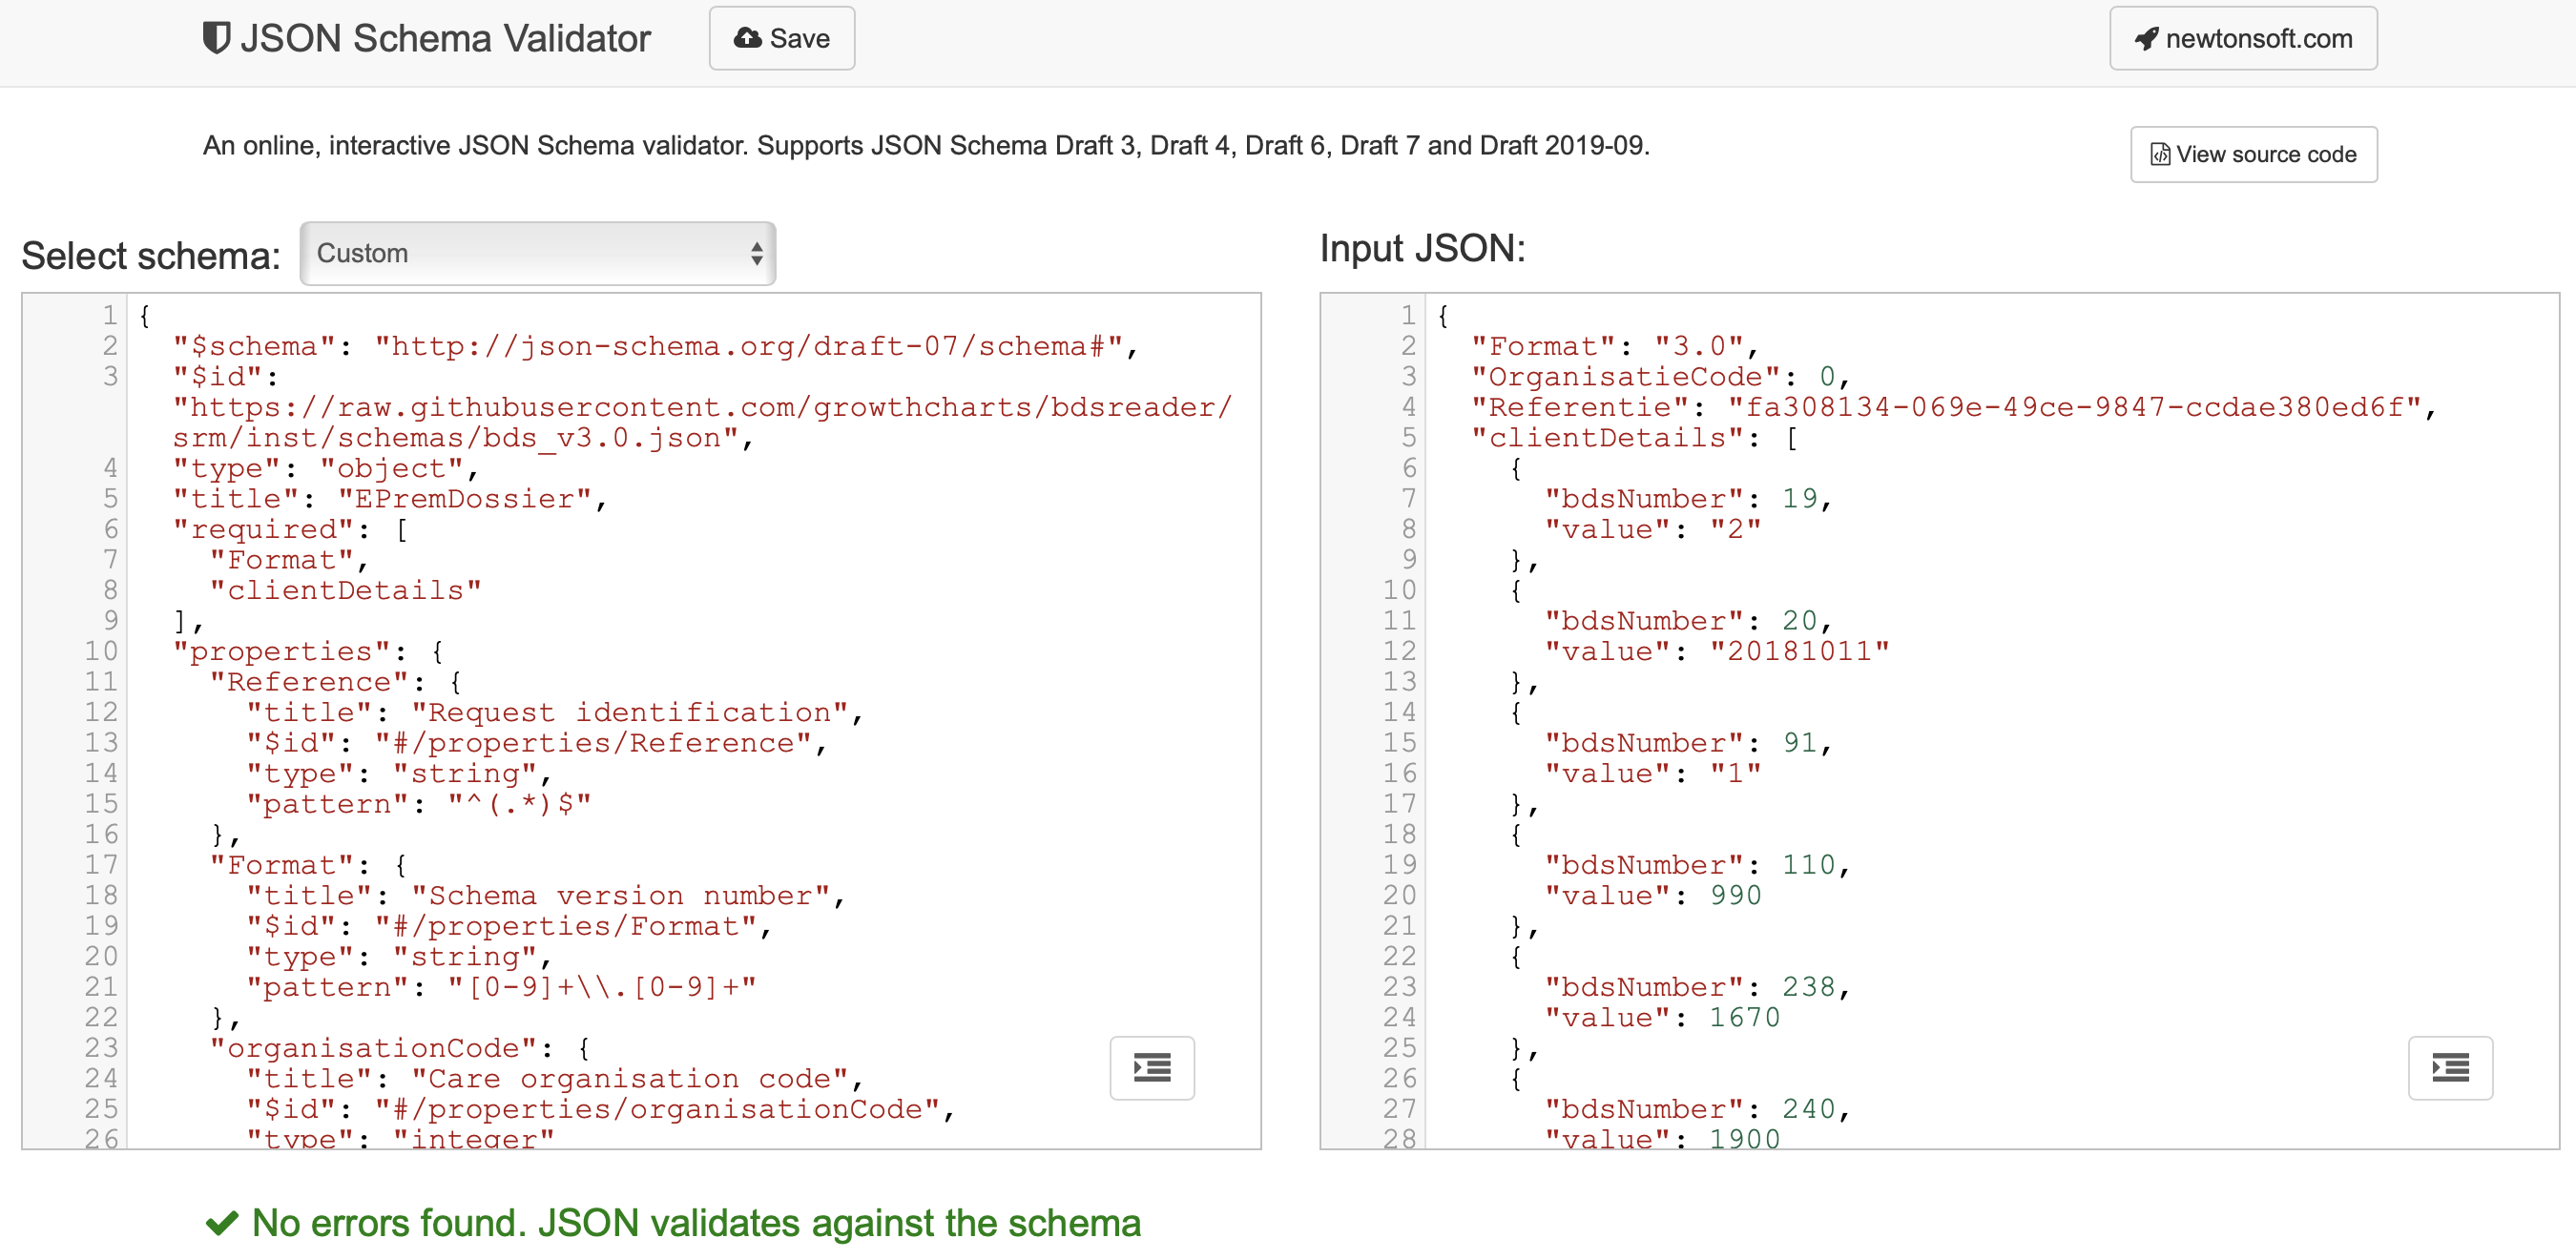
\includegraphics{fig/JSON-schema-validator.png}
\caption{\label{fig:jsonschema}Manual validation of a child dataset (right side) according JSON schema \texttt{bds\_v3.0.json}.}
\end{figure}



Experiment with your child file (e.g.~remove the required Format field) to see what types errors the validator can catch.

\hypertarget{bds-elements-supported-by-james}{%
\section{BDS-elements supported by JAMES}\label{bds-elements-supported-by-james}}

\begin{longtable}[]{@{}
  >{\raggedleft\arraybackslash}p{(\columnwidth - 8\tabcolsep) * \real{0.0811}}
  >{\raggedright\arraybackslash}p{(\columnwidth - 8\tabcolsep) * \real{0.3243}}
  >{\raggedleft\arraybackslash}p{(\columnwidth - 8\tabcolsep) * \real{0.0946}}
  >{\raggedright\arraybackslash}p{(\columnwidth - 8\tabcolsep) * \real{0.3514}}
  >{\raggedright\arraybackslash}p{(\columnwidth - 8\tabcolsep) * \real{0.1486}}@{}}
\toprule()
\begin{minipage}[b]{\linewidth}\raggedleft
BDS
\end{minipage} & \begin{minipage}[b]{\linewidth}\raggedright
Description
\end{minipage} & \begin{minipage}[b]{\linewidth}\raggedleft
Value
\end{minipage} & \begin{minipage}[b]{\linewidth}\raggedright
Label
\end{minipage} & \begin{minipage}[b]{\linewidth}\raggedright
\texttt{R} name
\end{minipage} \\
\midrule()
\endhead
19 & Sex of child & ``0'' & Unknown & \texttt{sex} \\
& & ``1'' & Male & \\
& & ``2'' & Female & \\
& & ``3'' & Not specified & \\
20 & Date of birth & ``yyyymmdd'' & year-month-day & \texttt{dob} \\
62 & Caretaker relation & ``01'' & biological father & \\
& & ``02'' & biological mother & \\
& & ``03'' & male partner, stepfather & \\
& & ``04'' & female partner, stepmother & \\
& & ``05'' & adoptive father & \\
& & ``06'' & adoptive mother & \\
& & ``07'' & foster father & \\
& & ``08'' & foster mother & \\
& & ``98'' & other & \\
63 & Caretaker date of birth & ``yyyymmdd'' & year-month-day & \texttt{dobf} \\
& & & & \texttt{dobm} \\
& & & & \texttt{agem} \\
66 & Caretaker education & ``01'' & no primary school & \texttt{-} \\
& & ``02'' & primary school, special ed & \\
& & ``03'' & VSO-MLK/IVBO/VMBO-LWOO & \\
& & ``04'' & LBO/VBO/VMBO-BBL\&KBL & \\
& & ``05'' & MAVO/VMBO-GL\&TL & \\
& & ``06'' & MBO & \\
& & ``07'' & HAVO/VWO & \\
& & ``08'' & HBO/HTS/HEAO & \\
& & ``09'' & WO & \\
& & ``98'' & Other & \\
& & ``00'' & Unknown & \\
71 & Caretaker birth country & ``dddd'' & \href{https://publicaties.rvig.nl/dsresource?objectid=29b66cb2-02ef-4a11-baf4-316ae00d8fa1}{4-digit code, Table 34} & \texttt{etn} (always \texttt{NL}) \\
82 & Gestational age & ``ddd'' & in days & \texttt{gad} \\
91 & Smoking during pregnancy & ``1'' & yes & \texttt{smo} \\
& & ``2'' & no & \\
& & ``99'' & unknown & \\
110 & Birth weight & ``dddd'' & 3-4 digits, grammes & \texttt{bw} (g) \\
235 & Length/height & ``dddd'' & 3-4 digits, millimeters & \texttt{hgt} (cm) \\
245 & Body weight & ``dddddd'' & 3-6 digits, grammes & \texttt{wgt} (kg) \\
252 & Head circumference & ``ddd'' & 2-3 digits, millimeters & \texttt{hdc} (cm) \\
238 & Height biological mother & ``dddd'' & 3-4 digits, millimeters & \texttt{hgtf} (cm) \\
240 & Height biological father & ``dddd'' & 3-4 digits, millimeters & \texttt{hgtm} (cm) \\
510 & Passive smoking & ``01'' & No smoking in house & \texttt{-} \\
& & ``02'' & Never with child & \\
& & ``03'' & Not in last 7 days & \\
& & ``04'' & Yes & \\
\bottomrule()
\end{longtable}

JAMES supports the following BDS numbers with Van Wiechen items: 879, 881, 883, 884, 885, 887, 888, 889, 890, 891, 894, 896, 897, 898, 902, 903, 906, 907, 910, 912, 914, 916, 917, 918, 920, 922, 923, 926, 945, 951, 955, 956, 958, 959, 961, 962, 964, 966, 968, 970, 971, 973, 975, 977, 978, 986, 989, 991, 993, 994, 996, 999, 1002, 886, 892, 893, 900, 905, 909, 913, 921, 927, 928, 930, 931, 932, 933, 934, 935, 936, 937, 938, 939, 940, 941, 943, 947, 948, 949, 950, 953, 954, 972, 980, 982, 984, 998, 1001, 1278.

The results of the Van Wiechen items are converted into 0/1 codes (by \href{https://github.com/growthcharts/bdsreader/blob/master/R/convert_ddi_gsed.R}{bdsreader:::convert\_ddi\_gsed}) and stored with GSED 9-position names as defined by the \href{https://d-score.org/dscore/}{\texttt{dscore}} package.

In addition, JAMES reads the following non-BDS fields:

\begin{longtable}[]{@{}
  >{\raggedleft\arraybackslash}p{(\columnwidth - 6\tabcolsep) * \real{0.2687}}
  >{\raggedright\arraybackslash}p{(\columnwidth - 6\tabcolsep) * \real{0.3582}}
  >{\raggedleft\arraybackslash}p{(\columnwidth - 6\tabcolsep) * \real{0.2239}}
  >{\raggedright\arraybackslash}p{(\columnwidth - 6\tabcolsep) * \real{0.1493}}@{}}
\toprule()
\begin{minipage}[b]{\linewidth}\raggedleft
Fields
\end{minipage} & \begin{minipage}[b]{\linewidth}\raggedright
Description
\end{minipage} & \begin{minipage}[b]{\linewidth}\raggedleft
Type
\end{minipage} & \begin{minipage}[b]{\linewidth}\raggedright
\texttt{R} name
\end{minipage} \\
\midrule()
\endhead
Reference & Description (opt) & String & \texttt{name} \\
Format & JSON schema number (req) & Number.Number & \texttt{-} \\
organisationCode & Organisation code (opt) & Integer & \texttt{src} \\
\bottomrule()
\end{longtable}

\hypertarget{james-internal-data}{%
\section{JAMES internal data}\label{james-internal-data}}

Suppose we coded the following data set.

\begin{verbatim}
{
  "Format": "3.0",
  "organisationCode": 1234,
  "Reference": "Maria",
  "clientDetails": [
    {
      "bdsNumber": 19,
      "value": "2"
    },
    {
      "bdsNumber": 20,
      "value": "20181011"
    },
    {
      "bdsNumber": 82,
      "value": 189
    },
    {
      "bdsNumber": 91,
      "value": "1"
    },
    {
      "bdsNumber": 110,
      "value": 990
    },
    {
      "bdsNumber": 238,
      "value": 1670
    },
    {
      "bdsNumber": 240,
      "value": 1900
    }
  ],
  "clientMeasurements": [
    {
      "bdsNumber": 235,
      "values": [
        {
          "date": "20181111",
          "value": 380
        },
        {
          "date": "20181211",
          "value": 435
        }
      ]
    },
    {
      "bdsNumber": 245,
      "values": [
        {
          "date": "20181011",
          "value": 990
        },
        {
          "date": "20181111",
          "value": 1250
        },
        {
          "date": "20181211",
          "value": 2100
        }
      ]
    },
    {
      "bdsNumber": 252,
      "values": [
        {
          "date": "20181111",
          "value": 270
        },
        {
          "date": "20181211",
          "value": 305
        }
      ]
    }
  ],
  "nestedDetails": [
    {
      "nestingBdsNumber": 62,
      "nestingCode": "01",
      "clientDetails": [
        {
          "bdsNumber": 63,
          "value": "19950704"
        }
      ],
      "clientMeasurements": [

      ]
    },
    {
      "nestingBdsNumber": 62,
      "nestingCode": "02",
      "clientDetails": [
        {
          "bdsNumber": 63,
          "value": "19901202"
        }
      ],
      "clientMeasurements": [

      ]
    }
  ]
}
\end{verbatim}

The following R script shows reading and conversion of the data.

\begin{Shaded}
\begin{Highlighting}[]
\FunctionTok{library}\NormalTok{(bdsreader)}
\NormalTok{fn }\OtherTok{\textless{}{-}} \FunctionTok{system.file}\NormalTok{(}\StringTok{"examples/maria.json"}\NormalTok{, }\AttributeTok{package =} \StringTok{"bdsreader"}\NormalTok{)}
\NormalTok{m }\OtherTok{\textless{}{-}} \FunctionTok{read\_bds}\NormalTok{(fn)}
\end{Highlighting}
\end{Shaded}

Object \texttt{m} object is a list with two components:

\begin{itemize}
\tightlist
\item
  \texttt{m\$psn} a tibble with one row containing fixed covariates
\item
  \texttt{m\$xyz} a tibble with multiple rows with time-varying data
\end{itemize}

\begin{Shaded}
\begin{Highlighting}[]
\NormalTok{m}\SpecialCharTok{$}\NormalTok{psn}
\end{Highlighting}
\end{Shaded}

\begin{verbatim}
## # A tibble: 1 x 16
##      id name  dob        dobf       dobm       src   dnr   sex      gad    ga
##   <int> <chr> <date>     <date>     <date>     <chr> <chr> <chr>  <dbl> <dbl>
## 1    -1 Maria 2018-10-11 1995-07-04 1990-12-02 1234  <NA>  female   189    27
## # i 6 more variables: smo <int>, bw <dbl>, hgtm <dbl>, hgtf <dbl>, agem <dbl>,
## #   etn <chr>
\end{verbatim}

\begin{Shaded}
\begin{Highlighting}[]
\NormalTok{m}\SpecialCharTok{$}\NormalTok{xyz}
\end{Highlighting}
\end{Shaded}

\begin{verbatim}
## # A tibble: 11 x 8
##       age xname yname zname zref                        x     y      z
##     <dbl> <chr> <chr> <chr> <chr>                   <dbl> <dbl>  <dbl>
##  1 0.0849 age   hgt   hgt_z nl_2012_hgt_female_27  0.0849 38    -0.158
##  2 0.0849 age   wgt   wgt_z nl_2012_wgt_female_27  0.0849  1.25 -0.203
##  3 0.0849 age   hdc   hdc_z nl_2012_hdc_female_27  0.0849 27    -0.709
##  4 0.0849 age   bmi   bmi_z nl_1997_bmi_female_nl  0.0849  8.66 -5.72 
##  5 0.167  age   hgt   hgt_z nl_2012_hgt_female_27  0.167  43.5   0.047
##  6 0.167  age   wgt   wgt_z nl_2012_wgt_female_27  0.167   2.1   0.015
##  7 0.167  age   hdc   hdc_z nl_2012_hdc_female_27  0.167  30.5  -0.913
##  8 0.167  age   bmi   bmi_z nl_1997_bmi_female_nl  0.167  11.1  -3.77 
##  9 0      age   wgt   wgt_z nl_2012_wgt_female_27  0       0.99  0.19 
## 10 0.0849 hgt   wfh   wfh_z nl_2012_wfh_female_   38       1.25 -0.001
## 11 0.167  hgt   wfh   wfh_z nl_2012_wfh_female_   43.5     2.1   0.326
\end{verbatim}

\hypertarget{growth-charts-in-james}{%
\chapter{Growth charts in JAMES}\label{growth-charts-in-james}}

\hypertarget{chart-naming-conventions}{%
\section{Chart naming conventions}\label{chart-naming-conventions}}

The link \url{https://groeidiagrammen.nl/ocpu/lib/james/www/} contains an interactive overview of the available growth charts. There are many different charts: for boys and girls, for preterms, for different age ranges, for specific ethnic groups, for height, weight, BMI, and so on. Each chart has a chart code, a character code identifying the design. This section explains the construction of the chart codes.

The GitHub repository \url{https://github.com/growthcharts/chartbox} contains the chart libraries that are available to JAMES. The \texttt{list\_charts()} function produces a tabular overview.

\begin{Shaded}
\begin{Highlighting}[]
\NormalTok{charts }\OtherTok{\textless{}{-}}\NormalTok{ chartbox}\SpecialCharTok{::}\FunctionTok{list\_charts}\NormalTok{()}
\FunctionTok{dim}\NormalTok{(charts)}
\end{Highlighting}
\end{Shaded}

\begin{verbatim}
## [1] 478   8
\end{verbatim}

\begin{Shaded}
\begin{Highlighting}[]
\NormalTok{charts[}\FunctionTok{c}\NormalTok{(}\DecValTok{1}\NormalTok{, }\DecValTok{22}\NormalTok{, }\DecValTok{23}\NormalTok{, }\DecValTok{300}\NormalTok{, }\DecValTok{301}\NormalTok{, }\DecValTok{340}\NormalTok{), ]}
\end{Highlighting}
\end{Shaded}

\begin{verbatim}
##     chartgrp chartcode population    sex design  side language week
## 1     nl2010      DJAA         DS   male      A front    dutch     
## 22    nl2010      DMBA         DS female      B front    dutch     
## 23    nl2010      DMBB         DS female      B  back    dutch     
## 300  preterm   PMAAN32         PT female      A front    dutch   32
## 301  preterm   PMAAN33         PT female      A front    dutch   33
## 340  preterm   PMAHN36         PT female      A   hgt    dutch   36
\end{verbatim}

The \texttt{chartbox} package currently contains three chart groups: \texttt{nl2010}, \texttt{preterm} and \texttt{who}. Each group collects charts of a similar type.

\begin{longtable}[]{@{}
  >{\raggedright\arraybackslash}p{(\columnwidth - 8\tabcolsep) * \real{0.0964}}
  >{\raggedleft\arraybackslash}p{(\columnwidth - 8\tabcolsep) * \real{0.0723}}
  >{\raggedright\arraybackslash}p{(\columnwidth - 8\tabcolsep) * \real{0.1325}}
  >{\raggedright\arraybackslash}p{(\columnwidth - 8\tabcolsep) * \real{0.5783}}
  >{\raggedright\arraybackslash}p{(\columnwidth - 8\tabcolsep) * \real{0.1205}}@{}}
\toprule()
\begin{minipage}[b]{\linewidth}\raggedright
Chart Group
\end{minipage} & \begin{minipage}[b]{\linewidth}\raggedleft
N
\end{minipage} & \begin{minipage}[b]{\linewidth}\raggedright
Chart code
\end{minipage} & \begin{minipage}[b]{\linewidth}\raggedright
Description
\end{minipage} & \begin{minipage}[b]{\linewidth}\raggedright
Source
\end{minipage} \\
\midrule()
\endhead
\texttt{nl2010} & 140 & CCCC & Dutch children 0-21 years, including minorities & \citet{talma2010} \\
\texttt{preterm} & 240 & CCCCCNN & Dutch preterms, ga \textless= 36 weeks, 0-4 years & \citet{bocca2012} \\
\texttt{who} & 14 & CCCC & WHO Child Growth Standards 0-4 years & \href{https://www.who.int/childgrowth/en/}{WHO} \\
\bottomrule()
\end{longtable}

The chart code is an alpha-numeric code of four (for \texttt{nl2010} and \texttt{who}) or seven (for \texttt{preterm}) that uniquely identifies each of the charts. The table below specifies the full coding schema used to construct the chart codes.

\begin{longtable}[]{@{}clll@{}}
\toprule()
Position & Field & Value & Description \\
\midrule()
\endhead
1 & Population & N & Dutch \\
& & T & Turkish \\
& & M & Moroccan \\
& & H & Hindostan \\
& & P & Preterm \\
& & W & WHO \\
2 & Sex & J & Male \\
& & M & Female \\
3 & Design & A & 0-15 months \\
& & B & 0-4 years, WFH \\
& & C & 1-21 years \\
& & D & 0-21 years \\
& & E & 0-4 years, WFA \\
4 & Side & A & A4, front \\
& & B & A4, back \\
& & C & A4, back, no \texttt{hdc} \\
& & D & square, \texttt{dsc} \\
& & H & square, \texttt{hgt} \\
& & O & square, \texttt{hdc} \\
& & Q & square, \texttt{bmi} \\
& & R & square, \texttt{wfh} \\
& & W & square, \texttt{wgt} \\
& & X & A4, double sided \\
5 & Language & N & Dutch \\
& & E & English \\
6-7 & Week & 25-36 & Gestational age \\
\bottomrule()
\end{longtable}

For illustration, code \texttt{NJAA} references to Dutch (\texttt{N}), boys (\texttt{J}), 0-15 month (\texttt{A}), front side (\texttt{A}). Likewise, \texttt{PMEAN33} codes for the chart of preterm (\texttt{M}), girls (\texttt{M}), 0-4 years (\texttt{E}), front side (\texttt{A}), Dutch language (\texttt{N}) born at 33 weeks of gestation (\texttt{33}).

Some forms hold multiple growth charts. For example, the \texttt{NJAA} chart is designed for A4 paper size (297mm \(\times\) 210mm) and contains three growth charts: head circumference by age, length by age, and weight by age. Some others have no diagram, like \texttt{NJAB}. All square formats hold just one growth chart. All of the square forms have equal sizes (160mm \(\times\) 160mm).

The following table lists the measures per design-form combination.

\begin{longtable}[]{@{}ccll@{}}
\toprule()
Design & Side & Measure & Description \\
\midrule()
\endhead
A & A & \texttt{hdc} & Head circumference by age, 0-15 mo \\
& & \texttt{hgt} & Length by age, 0-15 mo \\
& & \texttt{wgt} & Weight by age, 0-15 mo \\
& B & & Backside explanations \\
& D & \texttt{dsc} & D-score by age, 0-15 mo \\
& H & \texttt{hgt} & Length by age, 0-15 mo \\
& O & \texttt{hdc} & Head circumference by age, 0-15 mo \\
& W & \texttt{wgt} & Weight by age, 0-15 mo \\
B & A & \texttt{wfh} & Weight for height, 0-4 yr \\
& & \texttt{hgt} & Length by age, 0-4 yr \\
& B & \texttt{hdc} & Head circumference by age, 0-4 yr \\
& C & & Backside explanations \\
& D & \texttt{dsc} & D-score by age, 0-4 yr \\
& H & \texttt{hgt} & Height by age, 0-4 yr \\
& O & \texttt{hdc} & Head circumference by age, 0-4 yr \\
& R & \texttt{wfh} & Weight for height, 0-4 yr \\
& W & \texttt{wgt} & Weight by age, 0-4 yr \\
C & A & \texttt{wfh} & Weight for height, 1-21 yr \\
& & \texttt{hgt} & height by age, 1-21 yr \\
& B & \texttt{bmi} & BMI by age, 1-21 yr \\
& & \texttt{hdc} & Head circumference by age, 1-21 yr \\
& C & \texttt{bmi} & BMI by age, 1-21 yr \\
& H & \texttt{hgt} & Height by age, 1-21 yr \\
& O & \texttt{hdc} & Head circumference by age, 1-21 yr \\
& Q & \texttt{bmi} & Body mass index by age, 1-21 yr \\
& R & \texttt{wfh} & Weight for height, 1-21 yr \\
E & A & \texttt{wgt} & Weight by age, 0-4 yr \\
& & \texttt{hgt} & height by age, 0-4 yr \\
& B & \texttt{hdc} & Head circumference by age, 0-4 yr \\
& H & \texttt{hgt} & Height by age, 0-4 yr \\
& O & \texttt{hdc} & Head circumference by age, 0-4 yr \\
& W & \texttt{wgt} & Weight by age, 0-4 yr \\
\bottomrule()
\end{longtable}

\hypertarget{methods}{%
\chapter{Methods}\label{methods}}

We describe our methods in this chapter.

\hypertarget{d-score-implementation}{%
\chapter{D-score implementation}\label{d-score-implementation}}

This document describes the actions taken to implement the \href{https://d-score.org/dbook1/}{D-score} into JAMES. The functionality of JAMES is distributed over multiple packages. This set of actions may be of interest when implementing new features.

\hypertarget{actions}{%
\section{Actions}\label{actions}}

\begin{longtable}[]{@{}
  >{\raggedright\arraybackslash}p{(\columnwidth - 4\tabcolsep) * \real{0.2857}}
  >{\raggedright\arraybackslash}p{(\columnwidth - 4\tabcolsep) * \real{0.3214}}
  >{\raggedright\arraybackslash}p{(\columnwidth - 4\tabcolsep) * \real{0.3929}}@{}}
\toprule()
\begin{minipage}[b]{\linewidth}\raggedright
Package
\end{minipage} & \begin{minipage}[b]{\linewidth}\raggedright
PR
\end{minipage} & \begin{minipage}[b]{\linewidth}\raggedright
Description
\end{minipage} \\
\midrule()
\endhead
minihealth & \href{https://github.com/growthcharts/minihealth/commit/03a32f1960e81a685bb749911e6ea297684ab4dc}{03a32f1} & Create milestones descriptions \\
dscore & \href{https://github.com/D-score/dscore/commit/f0013ce9a02d34ad25dd5c101c6a7c5b1444b53b}{f0013ce} & Link BDS number to Van Wiechen milestones \\
dscore & \href{https://github.com/D-score/dscore/commit/688685477082ac6c040b9d18035b5178a39a5cc0}{6886854} & Fine tuning of milestone labels \\
minihealth & & Create the \texttt{bds\_lexicon} object \\
minihealth & \href{https://github.com/stefvanbuuren/minihealth/commit/4893982631717539b070c8d19b88b2b10319f2ee}{4893982} & Add milestones to BDS validation JSON schema \\
minihealth & \href{https://github.com/stefvanbuuren/minihealth/commit/0069671c8d09f64f2436faa93b764bd288324fcc}{0069671} & Add \texttt{convert\_ddi\_gsed()} to convert BDS-milestones into GSED items \\
minihealth & \href{https://github.com/stefvanbuuren/minihealth/commit/8ab1392fdbe781adfa004fcadb4f661c14487cf2}{8ab1392} & Add a new class \texttt{individualDS} for storing milestones, D-score and DAZ \\
clopus & \href{https://github.com/stefvanbuuren/clopus/commit/1182cb02508a3207c0c9bcb35232851c38d24179}{1182cb0} & Add Dutch and GCDG D-score references \\
clopus & \href{https://github.com/stefvanbuuren/clopus/commit/7bdbcd9629bb215f466bbc2e2f886b6f16c5b5e9}{7bdbcd9} & Construct age-shifted D-score references for preterms \\
clopus & \href{https://github.com/stefvanbuuren/clopus/commit/ceab7f9547b9ae843a97b640d920ea0c36185053}{ceab7f9} & Import the D-score references into \texttt{clopus} \\
chartdesigner & \href{https://github.com/stefvanbuuren/chartdesigner/commit/68831906cef5cdca0d8851b057a01cc8be4fff6d}{6883190} & Add chart constructor functions for D-score, both terms and pre-terms \\
chartdesigner & \href{https://github.com/stefvanbuuren/chartdesigner/commit/511f456884bc62d6bebc9b5ef33cebb940dc126d}{511f456} & Extend internal \texttt{set.axes.design()} to D-score charts \\
chartdesigner & \href{https://github.com/stefvanbuuren/chartdesigner/commit/6582af8753331a25d8970683d4523c69d6959f0d}{6582af8} & Extend to \texttt{axes.locations} object to D-score charts \\
chartdesigner & \href{https://github.com/stefvanbuuren/chartdesigner/commit/47e3cc39d1253a41d3cc81d3d6dd55bffa842f18}{47e3cc3} & Create \texttt{dchart()} function and extend its helper functions \\
chartdesigner & \href{https://github.com/stefvanbuuren/chartdesigner/commit/fbbc7c8647ea010b2292fa9dd9b253ce95b6a54b}{fbbc7c8} & Function \texttt{chartcode()} factory, make one function for each chart code \\
chartcatalog & \href{https://github.com/growthcharts/chartcatalog/commit/cc467888dd5346d7ed2c0a78b976a8fa818f712c}{cc46788} & Extend the chart naming system to D-score charts \\
chartcatalog & \href{https://github.com/growthcharts/chartcatalog/commit/84aaded206a5050660bd347d2e093af93b6b7ae1}{84aaded} & Extend the lookup table \texttt{ynames\_lookup} to handle new D-score charts \\
chartbox & \href{https://github.com/growthcharts/chartbox/commit/aa310672a717f9777e2daac409d5ec40f3db509f}{aa31067} & Extend chart box with all D-score charts \\
james & \href{https://github.com/growthcharts/james/commits/dscore}{6412840} & Add radio button for D-score charts \\
minihealth & \href{https://github.com/stefvanbuuren/minihealth/commit/06a04c9ce70546db7998de5147a15897af0c7ddb}{06a04c9} & Calculate D-score and DAZ \\
chartplotter & \href{https://github.com/growthcharts/chartplotter/commit/4b5863813da5304ab5117feba216b7a0822fcd16}{4b58638} & Skip the \texttt{dsc} field for finding matches \\
minihealth & \href{https://github.com/stefvanbuuren/minihealth/commit/816be33b8921ab8d80d8a750d5c4e11966a58c18}{816be33} & Add D-score and DAZ to class \texttt{individualAN} \\
donordata & \href{https://github.com/stefvanbuuren/donordata/commit/77e01b40e2be75c19f27423092aa5626b0d5d3c3}{77e01b4} & Add milestones to SMOCC donor data \\
donordata & \href{https://github.com/stefvanbuuren/donordata/commit/ecb3413b115c3193135b1af118597768b083dc41}{ecb3413} & Calculate D-score and DAZ for SMOCC data \\
donordata & \href{https://github.com/stefvanbuuren/donordata/commit/3fa9d4de347d09ccff32a887cf6bd8dadfdfaeb6}{3fa9d4d} & Fit and store brokenstick model for D-score on SMOCC data \\
donorloader & \href{https://github.com/growthcharts/donorloader/commit/c22c44607b40ff6bda2009c25894362b68831275}{c22c446} & Update internal data after changes in donordata \\
jamesdocs & TBD & Document steps (this file) \\
donordata & \href{https://github.com/stefvanbuuren/donordata/commit/7983c3d81a69eb9c6b81a3e0f0668e892c5abf5a}{7983c3} & Saves the item scores to create JSON files \\
donordata & \href{https://github.com/stefvanbuuren/donordata/commit/1537182a0df4180e0000d59225c6355a9c506472}{1537182} & Save mapping between SMOCC and BDS coding scheme \\
donorloader & \href{https://github.com/growthcharts/donorloader/commit/e9a8ed9054ebe1ba3a060883d53cfa0ce1f963d2}{e9a8ed} & Make \texttt{smocc\_bds} available to JAMES \\
jamestest & \href{https://github.com/growthcharts/jamesdemo/commit/6484191fd8de0d93b35354aa3ee846447aa81df6}{648419} & Regenerate smocc JSON files to include DDI scores \\
jamestest & \href{https://github.com/growthcharts/jamesdemo/commit/ce1dbe5591ca7182fef05ea6c5cb0d1361e876dc}{ce1dbe} & Update the \texttt{installed.cabinets} object with the new individual milestones data \\
minihealth & \href{https://github.com/stefvanbuuren/minihealth/commit/4dda8daabca8811a4cc321c66aaccf31c4aba83f}{4dda8d} & Add class \texttt{individualRW} to store and convert raw milestones data \\
minihealth & \href{https://github.com/stefvanbuuren/minihealth/commit/9e03e7e39b007a9687d21efbaa13e77283866d5c}{9e03e7} & Complete the JSON validator schema \\
\bottomrule()
\end{longtable}

\hypertarget{opencpu-deployment}{%
\chapter{OpenCPU deployment}\label{opencpu-deployment}}

\hypertarget{objective-1}{%
\section{Objective}\label{objective-1}}

This chapter describes how to install JAMES on the server that run OpenCPU. This is the classic way to install and run OpenCPU applications, and has the advantage that AppArmor prevents various types of malicious behaviour. In the future, we will replace this procedure by containerised deployment using Docker.

\hypertarget{pre-requisites}{%
\section{Pre-requisites}\label{pre-requisites}}

\begin{itemize}
\tightlist
\item
  The server runs \texttt{Ubuntu\ 18.04} (or later, not tested on Ubuntu 20.04).
\item
  The user needs sudo access to the server that run \texttt{OpenCPU}.
\end{itemize}

\hypertarget{installation-of-james-in}{%
\section{Installation of JAMES in}\label{installation-of-james-in}}

Here is a set of commands that removes R and its libraries, installs the latest
R fresh from source, install JAMES and puts the machine to work.

A lot can go wrong. Please be patient to check each step.

\begin{Shaded}
\begin{Highlighting}[]
\CommentTok{\#!/bin/bash}
\CommentTok{\# Re{-}install opencpu{-}server, R and the libs}

\CommentTok{\# make system up to date}
\FunctionTok{sudo}\NormalTok{ apt{-}get update}
\FunctionTok{sudo}\NormalTok{ apt{-}get upgrade}

\CommentTok{\# disable opencpu}
\FunctionTok{sudo}\NormalTok{ a2dissite opencpu}
\FunctionTok{sudo}\NormalTok{ apachectl restart}

\CommentTok{\# disable pubertyplot \& webtool (only on testserver)}
\FunctionTok{sudo}\NormalTok{ a2dissite puberty}
\FunctionTok{sudo}\NormalTok{ a2dissite webtool}
\FunctionTok{sudo}\NormalTok{ apachectl restart}

\CommentTok{\# save configuration files}
\FunctionTok{mkdir}\NormalTok{ conf}
\FunctionTok{cp} \AttributeTok{{-}rv}\NormalTok{ /etc/opencpu/ \textasciitilde{}/conf/}
\FunctionTok{cp} \AttributeTok{{-}rv}\NormalTok{ /etc/apache2/ \textasciitilde{}/conf/}

\CommentTok{\# uninstall opencpu server \& full}
\FunctionTok{sudo}\NormalTok{ apt{-}get purge opencpu{-}server}
\FunctionTok{sudo}\NormalTok{ apt{-}get purge opencpu{-}full}

\CommentTok{\# remove all R libs}
\ExtensionTok{R} \AttributeTok{{-}e} \StringTok{\textquotesingle{}.libPaths()\textquotesingle{}}
\FunctionTok{sudo}\NormalTok{ rm }\AttributeTok{{-}rf}\NormalTok{ /usr/local/lib/R/site{-}library}
\FunctionTok{sudo}\NormalTok{ rm }\AttributeTok{{-}rf}\NormalTok{ /usr/lib/R/site{-}library}
\FunctionTok{sudo}\NormalTok{ rm }\AttributeTok{{-}rf}\NormalTok{ /usr/lib/R/library}

\CommentTok{\# remove R}
\FunctionTok{sudo}\NormalTok{ apt{-}get purge r{-}base{-}core}
\FunctionTok{sudo}\NormalTok{ apt{-}get purge r{-}base}
\FunctionTok{sudo}\NormalTok{ apt{-}get autoremove}

\CommentTok{\# add backport repositories for Ubuntu packages required by some R packages}
\FunctionTok{sudo}\NormalTok{ add{-}apt{-}repository }\StringTok{\textquotesingle{}deb https://mirror.nl.datapacket.com/ubuntu/ bionic main\textquotesingle{}}
\FunctionTok{sudo}\NormalTok{ add{-}apt{-}repository }\StringTok{\textquotesingle{}deb{-}src https://mirror.nl.datapacket.com/ubuntu/ bionic main\textquotesingle{}}

\CommentTok{\# install R. See https://cran.r{-}project.org/bin/linux/ubuntu/}
\CommentTok{\# update indices}
\FunctionTok{sudo}\NormalTok{ apt update }\AttributeTok{{-}qq}
\CommentTok{\# install two helper packages we need}
\FunctionTok{sudo}\NormalTok{ apt install }\AttributeTok{{-}{-}no{-}install{-}recommends}\NormalTok{ software{-}properties{-}common dirmngr}
\CommentTok{\# import the signing key (by Michael Rutter) for these repo}
\FunctionTok{sudo}\NormalTok{ apt{-}key adv }\AttributeTok{{-}{-}keyserver}\NormalTok{ keyserver.ubuntu.com }\AttributeTok{{-}{-}recv{-}keys}\NormalTok{ E298A3A825C0D65DFD57CBB651716619E084DAB9}
\CommentTok{\# we use R 4.0 (however note this actually installs R 4.1!! (May 2021))}
\FunctionTok{sudo}\NormalTok{ add{-}apt{-}repository }\StringTok{\textquotesingle{}deb https://cloud.r{-}project.org/bin/linux/ubuntu bionic{-}cran40/\textquotesingle{}}
\CommentTok{\# in the future: use cran{-}41}
\FunctionTok{sudo}\NormalTok{ apt install r{-}base}
\CommentTok{\# install r{-}base{-}dev because we want to compile from source}
\FunctionTok{sudo}\NormalTok{ apt{-}get install r{-}base{-}dev}

\CommentTok{\# install opencpu{-}server}
\FunctionTok{sudo}\NormalTok{ add{-}apt{-}repository }\AttributeTok{{-}y}\NormalTok{ ppa:opencpu/opencpu{-}2.2}
\FunctionTok{sudo}\NormalTok{ apt{-}get update}
\FunctionTok{sudo}\NormalTok{ apt{-}get upgrade}
\FunctionTok{sudo}\NormalTok{ apt{-}get install }\AttributeTok{{-}y}\NormalTok{ opencpu{-}server}

\CommentTok{\# restart opencpu}
\FunctionTok{sudo}\NormalTok{ a2ensite opencpu}
\FunctionTok{sudo}\NormalTok{ apachectl restart}

\CommentTok{\# manually check https://vps.stefvanbuuren.nl/ocpu }
\CommentTok{\# or https://www.groeidiagrammen.nl/ocpu}

\CommentTok{\# install application package: pubertyplot {-} only on dev server}
\FunctionTok{sudo}\NormalTok{ R }\AttributeTok{{-}e} \StringTok{\textquotesingle{}install.packages("/home/stef/packages/pubertyplot\_1.3.tar.gz", repos = NULL)\textquotesingle{}}
\FunctionTok{sudo}\NormalTok{ a2ensite puberty}
\FunctionTok{sudo}\NormalTok{ apachectl restart}

\CommentTok{\# install application package: webtool {-} only on dev server}
\FunctionTok{sudo}\NormalTok{ R }\AttributeTok{{-}e} \StringTok{\textquotesingle{}install.packages("RMySQL")\textquotesingle{}}
\FunctionTok{sudo}\NormalTok{ R }\AttributeTok{{-}e} \StringTok{\textquotesingle{}install.packages("/home/stef/packages/webtool\_1.1.tar.gz", repos = NULL)\textquotesingle{}}
\FunctionTok{sudo}\NormalTok{ a2ensite webtool}
\FunctionTok{sudo}\NormalTok{ apachectl restart}

\CommentTok{\# install JAMES packages {-} this may take a while {-} you need the right priveledges}
\FunctionTok{sudo}\NormalTok{ R }\AttributeTok{{-}e} \StringTok{\textquotesingle{}install.packages("remotes")\textquotesingle{}}
\FunctionTok{sudo}\NormalTok{ R }\AttributeTok{{-}e} \StringTok{\textquotesingle{}remotes::install\_github("growthcharts/james")\textquotesingle{}}

\CommentTok{\# remove duplicate packages}
\CommentTok{\# evade errors: "namespace \textquotesingle{}vctrs\textquotesingle{} 0.3.6 is already loaded, but \textgreater{}= 0.3.8 is required"}
\FunctionTok{sudo}\NormalTok{ R }\AttributeTok{{-}e} \StringTok{\textquotesingle{}remove.packages(c("ellipsis", "pillar", "vctrs"), "/usr/lib/opencpu/library")\textquotesingle{}}

\CommentTok{\# copy back opencpu configuration for JAMES (if they were OK, otherwise tweak)}
\FunctionTok{sudo}\NormalTok{ rm }\AttributeTok{{-}rf}\NormalTok{ /etc/opencpu}
\FunctionTok{sudo}\NormalTok{ cp }\AttributeTok{{-}rv}\NormalTok{ \textasciitilde{}/conf/opencpu /etc/opencpu/}

\CommentTok{\# active JAMES}
\FunctionTok{sudo}\NormalTok{ apachectl restart}

\CommentTok{\# check on https://tnochildhealthstatistics.shinyapps.io/james\_tryout/ }

\CommentTok{\# clean up: delete \textasciitilde{}/conf/ after everything works}
\FunctionTok{rm} \AttributeTok{{-}rf}\NormalTok{ conf}
\end{Highlighting}
\end{Shaded}

\hypertarget{dockerfile-for-james}{%
\chapter{Dockerfile for JAMES}\label{dockerfile-for-james}}

\hypertarget{objective-2}{%
\section{Objective}\label{objective-2}}

This chapter describes how to build and deploy JAMES as a Docker container.

\hypertarget{pre-requisites-1}{%
\section{Pre-requisites}\label{pre-requisites-1}}

JAMES is currently constructed from a collection of \texttt{R} packages. The top-level package at \url{https://github.com/growthcharts/james} also defines a Javascript interface in the \texttt{inst/www} directory. Deployment of JAMES relies on the \texttt{OpenCPU} server. In principle, it is enough to install the \texttt{james} package on the \texttt{OpenCPU} server, and will also install all dependencies.

The following is needed to build and run a JAMES image:

\begin{itemize}
\item
  Permission to read from the following private repo's:

  \begin{itemize}
  \tightlist
  \item
    \texttt{growthcharts/chartplotter}
  \item
    \texttt{growthcharts/curvematching}
  \item
    \texttt{growthcharts/donorloader}
  \item
    \texttt{growthcharts/jamesdocker}
  \end{itemize}
\item
  If needed, a personal Github token with repo scope from \href{https://help.github.com/en/github/authenticating-to-github/creating-a-personal-access-token-for-the-command-line}{here}, Generate a token with only scope repo.
\item
  Install \texttt{Docker\ Desktop} on your local machine, and run some tutorials
\end{itemize}

\hypertarget{dockerfile}{%
\section{Dockerfile}\label{dockerfile}}

The Dockerfile is at \url{https://raw.githubusercontent.com/growthcharts/jamesdocker/master/Dockerfile}, which is located in the private repo \url{https://github.com/growthcharts/jamesdocker}. You need authentication to use this resource.

\begin{itemize}
\tightlist
\item
  Clone the \texttt{growthcharts/jamesdocker} repo to your machine
\item
  Set working directory to root of \texttt{jamesdocker}
\item
  If needed: Add the file \texttt{docker/opencpu\_config/Renviron} with contents \texttt{GITHUB\_PAT=fa2...} with your own GITHUB\_PAT.
\end{itemize}

\hypertarget{docker-commands}{%
\section{Docker commands}\label{docker-commands}}

Build the \texttt{james} image, type in a terminal

\begin{Shaded}
\begin{Highlighting}[]
\ExtensionTok{docker}\NormalTok{ build }\AttributeTok{{-}t}\NormalTok{ james .}
\end{Highlighting}
\end{Shaded}

This may takes a long time (30 minutes), in which the entire application is downloaded from various web-locations. After (hopefully successful) completion, check the image

\begin{Shaded}
\begin{Highlighting}[]
\ExtensionTok{docker}\NormalTok{ images }\AttributeTok{{-}a}
\end{Highlighting}
\end{Shaded}

If all is well, the top line is called \texttt{james}. Now run the container on your local machine:

\begin{Shaded}
\begin{Highlighting}[]
\ExtensionTok{docker}\NormalTok{ run }\AttributeTok{{-}t} \AttributeTok{{-}d} \AttributeTok{{-}p}\NormalTok{ 80:80 james}
\end{Highlighting}
\end{Shaded}

If the ports are already taken by other containers, stop and remove all containers:

\begin{Shaded}
\begin{Highlighting}[]
\ExtensionTok{docker}\NormalTok{ stop }\VariableTok{$(}\ExtensionTok{docker}\NormalTok{ ps }\AttributeTok{{-}a} \AttributeTok{{-}q}\VariableTok{)}
\ExtensionTok{docker}\NormalTok{ rm }\VariableTok{$(}\ExtensionTok{docker}\NormalTok{ ps }\AttributeTok{{-}a} \AttributeTok{{-}q}\VariableTok{)}
\end{Highlighting}
\end{Shaded}

Reissue the \texttt{docker\ run}, and the container should now run. Check by

\begin{Shaded}
\begin{Highlighting}[]
\ExtensionTok{docker}\NormalTok{ ps}
\end{Highlighting}
\end{Shaded}

which should list a container created from the \texttt{james} image.

If you want to enter the container use

\begin{Shaded}
\begin{Highlighting}[]
\ExtensionTok{docker}\NormalTok{ exec }\AttributeTok{{-}i} \AttributeTok{{-}t}\NormalTok{ 6c /bin/bash}
\end{Highlighting}
\end{Shaded}

where \texttt{6c} are the first two characters of the container ID.

Inside the container, check font matching of Arial as

\begin{Shaded}
\begin{Highlighting}[]
\ExtensionTok{fc{-}match}\NormalTok{ Arial}
\end{Highlighting}
\end{Shaded}

\hypertarget{checks-with-the-browser}{%
\section{Checks with the browser}\label{checks-with-the-browser}}

\begin{Shaded}
\begin{Highlighting}[]
\ExtensionTok{http://localhost}
\end{Highlighting}
\end{Shaded}

should show Apache2 Ubuntu default screen.

\begin{Shaded}
\begin{Highlighting}[]
\ExtensionTok{http://localhost/ocpu/test/}
\end{Highlighting}
\end{Shaded}

should show \texttt{OpenCPU} test page.

\begin{Shaded}
\begin{Highlighting}[]
\ExtensionTok{http://localhost/rstudio/}
\end{Highlighting}
\end{Shaded}

should start the Rstudio IDE - \emph{if installed} . Use \texttt{opencpu:opencpu} to log in.

\begin{Shaded}
\begin{Highlighting}[]
\ExtensionTok{http://localhost/ocpu/library/james/www/}
\end{Highlighting}
\end{Shaded}

should start the JAMES javascript interface.

See also \url{https://registry.hub.docker.com/r/opencpu/rstudio}

\hypertarget{security}{%
\section{Security}\label{security}}

\begin{enumerate}
\def\labelenumi{\arabic{enumi}.}
\tightlist
\item
  Don't use the intermediate container, since it will contain your token in \texttt{/.Renviron}. The latest (\texttt{james}) container does not hold your token, and can be shared.
\item
  The container is shielded from the machine on which it runs. However, the materials within the container are only protected by \texttt{R\_LIMITS}. In general, for production it is wise to add restriction on the \texttt{OpenCPU} server.
\end{enumerate}

\hypertarget{certificates}{%
\chapter{Certificates}\label{certificates}}

\hypertarget{objective-3}{%
\section{Objective}\label{objective-3}}

The use of \texttt{htpps} requires that Apache runs with proper and validated certificates. Users can assess the status of the certificate by clicking on the slot in the browser bar. Certificates are issues by a Certificate Authority (CA) and are valid for one year. The period of one year is just enough to forget how to install and update certificates. This text shows how to renew the certificate.

\hypertarget{vps.stefvanbuuren.nl}{%
\section{vps.stefvanbuuren.nl}\label{vps.stefvanbuuren.nl}}

The server runs \texttt{Ubuntu\ 18.04\ LTS}. The Apache configuration file \texttt{/etc/apache2/sites-enabled/default-ssl.conf} contains the following lines

\begin{Shaded}
\begin{Highlighting}[]
        \ExtensionTok{SSLCertificateFile}\NormalTok{  /etc/ssl/crt/vps.stefvanbuuren.nl.chained.crt}
        \ExtensionTok{SSLCertificateKeyFile}\NormalTok{   /etc/ssl/crt/vps.stefvanbuuren.nl.key}
\end{Highlighting}
\end{Shaded}

The file \texttt{.key} is the private key, which should not leave the machine and only be read/write by sudoers. The file \texttt{..chained.crt} is the certificate file, which needs to be updated after expiry. There is some hand work involved in creating this file.

\hypertarget{step-1-create-the-csr-file}{%
\subsection{Step 1: Create the CSR file}\label{step-1-create-the-csr-file}}

\begin{Shaded}
\begin{Highlighting}[]
\FunctionTok{ssh}\NormalTok{ into vps.stefvanbuuren.nl}
\BuiltInTok{cd}\NormalTok{ /etc/ssl/crt}
\ExtensionTok{openssl}\NormalTok{ req }\AttributeTok{{-}new} \AttributeTok{{-}newkey}\NormalTok{ rsa:2048 }\AttributeTok{{-}nodes} \AttributeTok{{-}keyout}\NormalTok{ vps.stefvanbuuren.nl.key }\AttributeTok{{-}out}\NormalTok{ vps.stefvanbuuren.nl.csr}
\end{Highlighting}
\end{Shaded}

You need to answer some questions (See \url{http://edtechchris.com/2020/02/11/generate-csr-with-openssl-on-ubuntu/}). Show the result:

\begin{Shaded}
\begin{Highlighting}[]
\FunctionTok{cat}\NormalTok{ vps.stefvanbuuren.nl.csr}
\end{Highlighting}
\end{Shaded}

Copy the contents of the CSR file onto the clipboard. Save also on desktop under \texttt{Package/james/certificates\_vps.stefvanbuuren.nl/\{expiryyear\}} for archiving.

\hypertarget{step-2-buy-new-certificate}{%
\subsection{Step 2: Buy new certificate}\label{step-2-buy-new-certificate}}

The current CA is Network Solutions. Log into their website, and pay their renewal fee (about \$86 per year). Select Apache/Ubuntu, paste CSR clipboard file into appropriate box, and submit.

Within 30 minutes you get a request to validate in the mailbox. After that is done, you get a new mail saying that certificates are available. Download everything.

\hypertarget{step-3-create-the-crt-file}{%
\subsection{Step 3: Create the crt file}\label{step-3-create-the-crt-file}}

Collect the following four files into \texttt{Package/james/certificates\_vps.stefvanbuuren.nl/\{expiryyear\}}.

\begin{Shaded}
\begin{Highlighting}[]
\ExtensionTok{dv\_chain.txt}
\ExtensionTok{DV\_NetworkSolutionsDVServerCA2.crt}
\ExtensionTok{DV\_USERTrustRSACertificationAuthority.crt}
\ExtensionTok{VPS.STEFVANBUUREN.NL.crt}
\end{Highlighting}
\end{Shaded}

Create a new file as follows:

\begin{itemize}
\tightlist
\item
  Open with text editor \texttt{dv\_chain.txt} and \texttt{VPS.STEFVANBUUREN.NL.crt}
\item
  Paste the contents of \texttt{VPS.STEFVANBUUREN.NL.crt} \emph{before} the contents of \texttt{dv\_chain.txt}. There will be three sections.
\item
  Save the result under file name \texttt{vps.stefvanbuuren.nl.chained.crt}
\end{itemize}

\hypertarget{step-4-transfer-to-server}{%
\subsection{Step 4: Transfer to server}\label{step-4-transfer-to-server}}

Copy the file onto the server, home directory, by \texttt{ftp}. Move it in place by

\begin{Shaded}
\begin{Highlighting}[]
\FunctionTok{sudo}\NormalTok{ mv vps.stefvanbuuren.nl.chained.crt /etc/ssl/crt/vps.stefvanbuuren.nl.chained.crt}
\end{Highlighting}
\end{Shaded}

This overwrites the expired certificate.

\hypertarget{step-5-restart-apache2}{%
\subsection{Step 5: Restart Apache2}\label{step-5-restart-apache2}}

If you changed \texttt{/etc/apache2/sites-enabled/default-ssl.conf} check for syntactic validity.

\begin{Shaded}
\begin{Highlighting}[]
\ExtensionTok{apachectl}\NormalTok{ configtest}
\end{Highlighting}
\end{Shaded}

If OK, then

\begin{Shaded}
\begin{Highlighting}[]
\FunctionTok{sudo}\NormalTok{ apachectl restart}
\end{Highlighting}
\end{Shaded}

If all is well, Apache restarts and uses the updated certificate.

\hypertarget{troubleshooting}{%
\subsection{Troubleshooting}\label{troubleshooting}}

If it doesn't work, check whether the results of the following statements are identical.

\begin{Shaded}
\begin{Highlighting}[]
\ExtensionTok{openssl}\NormalTok{ x509 }\AttributeTok{{-}noout} \AttributeTok{{-}modulus} \AttributeTok{{-}in}\NormalTok{ vps.stefvanbuuren.nl.chained.crt }\KeywordTok{|} \ExtensionTok{openssl}\NormalTok{ md5}
\FunctionTok{sudo}\NormalTok{ openssl rsa }\AttributeTok{{-}noout} \AttributeTok{{-}modulus} \AttributeTok{{-}in}\NormalTok{ vps.stefvanbuuren.nl.key }\KeywordTok{|} \ExtensionTok{openssl}\NormalTok{ md5}
\end{Highlighting}
\end{Shaded}

If not, there is a mismatch between private key and certificate. See \url{https://stackoverflow.com/questions/26191463/ssl-error0b080074x509-certificate-routinesx509-check-private-keykey-values?rq=1} for fixes.

For others errors, consult the standard log

\begin{Shaded}
\begin{Highlighting}[]
\FunctionTok{sudo}\NormalTok{ tail }\AttributeTok{{-}f}\NormalTok{ /var/log/apache2/error.log}
\end{Highlighting}
\end{Shaded}


  \bibliography{book.bib,packages.bib}

\end{document}
